\documentclass[aps,prb,superscriptaddress,nofootinbib]{revtex4}
\usepackage{amsfonts}
\usepackage{amsmath}
\usepackage{amssymb}
\usepackage{graphbox}
\usepackage{graphicx}
\usepackage{caption}
\usepackage{bm}
\usepackage{bbm}
\usepackage{cancel}
\usepackage{color}
\usepackage{mathrsfs}
\usepackage[colorlinks,bookmarks=true,citecolor=blue,linkcolor=red,urlcolor=blue]{hyperref}
\usepackage{simpler-wick}
\usepackage{appendix}
\usepackage{float}
\usepackage{array}
\usepackage{booktabs}
\usepackage[export]{adjustbox}
\setlength{\parindent}{10 pt}
\setlength{\parskip}{2 pt}
\setcounter{MaxMatrixCols}{30}
\bibliographystyle{apsrev}
\newcommand{\RNum}[1]{\uppercase\expandafter{\romannumeral #1\relax}}
\newcommand{\normord}[1]{{:\mathrel{#1}:}}
\def\tbs{\textbackslash}
\def \tr{\operatorname{tr}}
\def \Tr{\operatorname{Tr}}


\begin{document}
\title{Conformal Field Theory}
\author{Jie Ren}


\maketitle


\tableofcontents

\section{The Conformal Invariance}


\subsection{Conformal algebra in 2D}
A \textit{conformal transformation} changes the metric by $g_{\mu\nu}(x) \rightarrow \Omega(x) g_{\mu\nu}(x)$.\footnote{We focus on the flat Euclidean space, where we use the $\eta_{\mu\nu} = \delta_{\mu\nu}$ to denote the metric.}
For $d=2$, the coordinate can be mapped to the complex plane by $z = x^0 + i x^1$, and the conformal transformations coincide with the analytic coordinate transformations $z \rightarrow f(z)$, $\bar z\rightarrow \bar f(\bar z)$.
Now consider the infinitesimal local conformal transformations:
\begin{equation}
	z \rightarrow z' = z + \sum_{n\in\mathbb Z} c_n \epsilon_n(z),\quad
	\bar z \rightarrow \bar z' = \bar z + \sum_{n\in\mathbb Z} \bar c_n \bar\epsilon_n(\bar z),\quad
	\epsilon_n(z) = z^{n+1},\quad 
	\bar\epsilon_n(\bar z) = \bar z^{n+1}.
\end{equation}
Under the infinitesimal coordinate transformation, a spinless, dimensionless field $\phi(z,\bar z)$ becomes $\phi'(z',\bar z')$, satisfying
\begin{equation}
	\phi'(z',\bar z') = \phi(z=z'-\epsilon,\bar z=\bar z'-\bar \epsilon) = \phi(z',\bar z')-(\epsilon\partial_{z}+\bar\epsilon\partial_{\bar z})\phi(z',\bar z').
\end{equation}
The variation of $\phi(z)$ under infinitesimal conformal transformation is
\begin{equation}
	\delta_{\epsilon,\bar\epsilon} \phi(z,\bar z)\equiv \phi'(z,\bar z)-\phi(z,\bar z) = -\epsilon\partial_{z}\phi(z',\bar z')-\bar\epsilon\partial_{\bar z}\phi(z',\bar z')
	\equiv \sum_{n\in \mathbb Z} \left(c_n l_n +\bar c_n \bar l_n\right)\phi(z,\bar z).
\end{equation}
The corresponding generators are $l_n = -z^{n+1}\partial_z$ and $\bar l_n = -\bar z^{n+1}\partial_{\bar z}$, satisfying the comutation algebra
\begin{equation}\label{eq:cls-cft-gens}
	\left[l_n, l_m\right] = (n-m)l_{m+n},\quad
	\left[\bar l_n, \bar l_m\right] = (n-m) \bar l_{m+n},\quad
	\left[l_n, \bar l_m\right] = 0.
\end{equation}
In the quantum case, the algebra (\ref{eq:cls-cft-gens}) will be central extended to the \textit{Virasoro algebra} which includes an extra term proportional to a \textit{central charge}:
\begin{equation}\label{eq:virasoro-algebra}
	\left[L_n, L_m\right] = (n-m) L_{m+n} + \frac{c}{12}(n-1)n(n+1)\delta_{m+n,0}.
\end{equation}
Since $l_n$'s commute with $\bar l_m$'s, the local conformal algebra is the direct sum $\mathcal{A}\oplus\bar{\mathcal{A}}$.
Since the algebra is independent, it is useful to regard $z$ and $\bar z$ as independent coordinates.
A more formal statement is that since the action of the conformal group factorizes into independent action of $z$ and $\bar z$, correlation functions of 2D CFT can be analytically continued to a larger domain which, in terms of the original coordinate $(x^0,x^1)$, amounts to taking $(x^0,x^1)\in \mathbb C^2$.
In $\mathbb C^2$, the surface defined by $\bar z = z^*$ is called the \textit{real surface}.
This procedure allows the algebra $\mathcal{A}\oplus\bar{\mathcal A}$ to act on $\mathbb C^2$, and the ``physical" condition $\bar z = z^*$ is left to be imposed at our convenience.
The real condition is preserved by the subalgebra of $\mathcal{A}\oplus\bar{\mathcal A}$ genrated by $l_n+\bar l_n$ and $i(l_n-\bar l_n)$.
In the following, we shall use the independence of the algebra to just ignore the anti-holomorphic dependence for simplicity.

We call Eq.~(\ref{eq:cls-cft-gens}) local transformation because not all of them are globally well-defined.\footnote{A globally well defined $f(z)$ is analytic on the Riemann sphere $\mathbb C\cup \infty$, i.e., $f(z)$ not only has no pole on the complex plane but also behaves non-singularly as $z\rightarrow \infty$. The latter condition is equivalent to non-singularity for $f(1/z)$ at $z=0$.}
The global conformal transformation is generated by $\{l_{-1},l_0,l_1\}\cup\{\bar l_{-1},\bar l_0,\bar l_1\}$.
We identify $l_{-1}$, $\bar l_{-1}$ as generators of translations, $l_{0}+\bar l_{0}$, $i(l_{0}-\bar l_{0})$ as generators of dilations and rotations resplectively, $l_{1}$, $\bar l_{1}$ as generators of special conformal transformations (SCTs).
A compact form for these transformations is
\begin{equation}
	z \rightarrow f(z) = \frac{a z + b}{c z + d},\quad ad-bc = 1.
\end{equation}
This type of mapping is called \textit{projective transformations}, and to each of them we can associate a $2\times2$ matrix:
\begin{equation}
	A = \begin{bmatrix} a & b \\ c & d \end{bmatrix}: \quad
	A_\text{trn} = \begin{bmatrix} 1 & b \\ 0 & 1 \end{bmatrix}, \quad
	A_\text{rot} = \begin{bmatrix} e^{i\theta/2} & 0 \\ 0 & e^{-i\theta/2} \end{bmatrix}, \quad
	A_\text{dil} = \begin{bmatrix} \lambda & 0 \\ 0 & \lambda^{-1} \end{bmatrix}, \quad
	A_{\mathrm{SCT}}(b) = \begin{bmatrix} 1 & 0 \\ b & 1 \end{bmatrix}.
\end{equation}

The global conformal algebra $\{l_{-1},l_0,l_1\}\cup\{\bar l_{-1},\bar l_0,\bar l_1\}$ is also useful to characterize properties of physical states.
It is a convention to work in the basis of eigenstates of $l_0$ and $\bar l_0$, and denote the eigenvalues as $h$ and $\bar h$ respectively.
Since $l_{0}+\bar l_{0}$ and $i(l_{0}-\bar l_{0})$ generate dilations and rotations respectively, the scaling dimension $\Delta$ and the spin $s$ of the state are given by $\Delta=h+\bar h$ and $s = h-\bar h$.

In the following, we will focus on the spinless case where $\Delta = 2h$.
A \textit{primary state} $|\nu\rangle$ with eigenvalue $h$ is a state such that 
\begin{equation}
	L_0|\nu\rangle = h|\nu\rangle,\quad
	L_{n>0} |\nu\rangle = 0.
\end{equation}
All the remaining weights are in the form of $\{L_{-n_1}\cdots L_{-n_k}|\nu\rangle\}$.
The primary state and its descendants form a \textit{Verma module} $\mathscr V_h$.\footnote{We implicitly assume $|\nu\rangle$ is also primary for $\{\bar L_n\}$, with conformal dimension $\bar h=h$.}
Note that for certain values of $h$, the Verma modules may be reducible.
First consider the $k=2$ level, where a state can be parametrized as $|\chi\rangle = (L_{-2} + \eta L_{-1}^2)|\nu\rangle$.
The condition for $|\chi\rangle$ to to primary is
\begin{equation}
	L_1|\chi\rangle = L_2|\chi\rangle = 0 
	\quad \Longrightarrow \quad 
	h_\pm = \frac{5-c\pm\sqrt{(c-1)(c-25)}}{16},\ 
	\eta=-\frac{3}{2(2h+1)}.
\end{equation}
We may simplify the notation by (which also generalizes the solution to $N=rs$ level)
\begin{equation}
	h_{r,s} = \frac{c-1}{24} + \frac{(r\alpha_+ + s \alpha_-)^2}{4}, \quad
	\alpha_\pm = \frac{\sqrt{1-c}\pm\sqrt{25-c}}{\sqrt{24}},\ 
	h_+ =\Delta_{2,1},\ h_-=\Delta_{1,2}.
\end{equation}
This can be shown that the coset module $\mathscr R_{r,s} \equiv \mathscr V_{h_{r,s}}/\mathscr V_{h_{r,s}+rs}$ is irreducible.
In the $\mathscr R_{r,s}$ module, the sub-primary state $L_{r,s}|\nu\rangle$ is called the \textit{null vector}.
We will see in the following that a conformal theory with a null vector imposes further constraints on the correlation function.

\subsection{Radial quantization}

In this section, we are going to construct the Hilbert space of the conformal field theory.
First, in conformal field theory, we identify the state and field.
That is, for every primary state $|w\rangle$, there is an associated field operator $\phi_{|w\rangle}$ such that
\begin{equation}
	|w\rangle = \phi_{|w\rangle}|0\rangle
	\quad\Longrightarrow\quad
	L_n|w\rangle = L_n\phi_{|w\rangle}|0\rangle,
\end{equation}
where $|0\rangle$ is the vacuum state invariant under all conformal transformations, i.e., $L_n|0\rangle=0$.
Second, the conserved charge of the conformal transformation generates the field variation:
\begin{equation}
	Q = \int dx\ j_t(x) = \int dx\ \left[\frac{1}{2\pi}T(z)\epsilon(z)\right]_t(x),\quad
	\delta_{\epsilon}\phi(z) = i \epsilon[Q,\phi(z)],
\end{equation}
where $T(z)$ is the stress tensor.
We choose radial direction as the time, in this way $z = \exp(t+ix)$ on the complex plane.\footnote{Equivalently, we may consider our theory on a finite spacetime cylinder, with time $-\infty$ to $+\infty$, and space from $0$ to $2\pi$ on a circle, in order to eliminate divergences.}
The equal-time surface, now being a circle, produce the variation:
\begin{equation}
	\delta_\epsilon \phi(z) = \oint\frac{dy}{2\pi i} \epsilon(y) \left[T(y),\phi(z)\right]
	= \mathcal T \left[\left(\oint_{|y|=|z|+\delta}-\oint_{|y|=|z|-\delta} \right) \frac{dy}{2\pi i} \epsilon(y)  T(y)\phi(z) \right]
	\simeq -\oint_z\frac{dy}{2\pi i} \epsilon(y) T(y)\phi(z),
\end{equation}
where in the last line, we adopt the convention that all bare operators really mean the time-ordered expectation.
On the other hand, the primary field transformed as
\begin{equation}
	\phi'_h(z') \rightarrow \left(\frac{\partial f}{\partial z}\right)^h \phi_h\left(f(z)\right)
	\quad\Longrightarrow\quad
	\delta_{\epsilon}\phi_{h}(z) = -\left[h \frac{\partial \epsilon}{\partial z}(z) +\epsilon(z) \frac{\partial}{\partial z}\right]\phi_{h}(z).
\end{equation}
Therefore, we know the operator product expansion (OPE):
\begin{equation}\label{eq:ope-1}
	T(y) \phi_{h}(z) = \frac{h \phi_{h}(z)}{(y-z)^2} +\frac{\partial \phi_{h}(z)}{y-z} +O(1),
\end{equation}
where we denote the regular terms by $O(1)$, and the time ordering is implicit. 
Note that the canonical definition of the stress tensor is
\begin{equation}
	T(z) = \sum_{n\in \mathbb Z}\frac{L_n}{z^{n+2}}
	\quad\Longrightarrow\quad
	L_n\phi(0) = \oint \frac{dy}{2\pi i} y^{n+1}T(y)\phi(0).
\end{equation}
This definition of $T(Z)$ is for the state $\phi(0)|0\rangle$ created at the remote past.
For generic $z$, we can shift the origin, and then a similar definition gives the action of $T(y)$ on the field $\phi(z)$:
\begin{equation}
	T(y) \phi(z) = \sum_{n \in \mathbb{Z}} \frac{L_n \phi(z)}{(y-z)^{n+2}} \quad \Longleftrightarrow\quad
	L_n \phi(z) = \oint_z \frac{dy}{2 \pi i} (y-z)^{n+1} T(y) \phi(z).
\end{equation}
For a primary field $\phi_h(z)$, this definition reduces to Eq.~(\ref{eq:ope-1}).
Also, two stress tensor has the OPE:
\begin{equation}\label{eq:ope-2}
	T(y) T(z) = \frac{c/2}{(y-z)^4} + \frac{2T(z)}{(y-z)^2} + \frac{\partial T(z)}{y-z} + O(1),
\end{equation}
which is similar to a primary field, but with an additional singular term proportional to the central charge.
To see this, consider the commutator of $L_n$'s:
\begin{equation}
\begin{aligned}
	\left[L_n, L_m\right]
	&= \oint_0 \frac{dy}{2\pi i}\ y^{m+1}\oint_y \frac{dz}{2\pi i}\ z^{n+1} \left[\frac{c/2}{(z-y)^4} + \frac{2T(y)}{(z-y)^2} + \frac{\partial T(y)}{z-y}\right] \\
	&= \oint_0 \frac{dy}{2\pi i}\ y^{m+n-1}\left[\frac{c (n-1)n(n+1)}{12} + 2(n+1)T(y)y^2 + y^3 \partial T(y) \right] \\
	&= \frac{c(n-1)n(n+1)}{12} \delta_{m+n,0} + (n-m) L_{m+n}.
\end{aligned}
\end{equation}
That is, Eq.~(\ref{eq:ope-2}) is equivalent to the Virasoro algebra.

For $N$ primary fields, we denote the correlation function as 
\begin{equation}
	Z \equiv \left\langle \phi_{h_1}(z_1)\cdots\phi_{h_N}(z_N)\right\rangle,\quad
	Z(y)\equiv \left\langle T(y) \phi_{h_1}(z_1)\cdots\phi_{h_N}(z_N)\right\rangle,
\end{equation}
where $Z(y)$ is a meromorphic function of $y$ with poles at $y=z_i$. 
The correlation function is invariant under the coordinate transformation: $\delta_{\epsilon}Z=0$, so that
\begin{equation}
	\sum_{i=1}^N \left[h \frac{\partial \epsilon}{\partial z}(z) +\epsilon(z) \frac{\partial}{\partial z}\right]Z = 0 
	\quad\Longrightarrow\quad
	\sum_{i=1}^N \left[n h z^{n-1} +z^n \frac{\partial}{\partial z}\right]Z = 0.
\end{equation}
For two-point function $\langle\phi_{h_1}(z_1)\phi_{h_2}(z_2)\rangle$, the first condition $(\partial_{z_1}+\partial_{z_2})Z=0$ requires translational invariants, which implies that $Z$ is a function of ($z_1-z_2$).
The second identity encodes scale invariance, which further restricts 
\begin{equation}
	\langle\phi_{h_1}(z_1)\phi_{h_2}(z_2)\rangle = \frac{C_{h_1h_2}}{(z_1-z_2)^{2h}},
\end{equation}
where a consistent solution requires $h_1=h_2=h$.
So a two-point function can be non-vanishing only if the two fields have the same dimension. 
For three-point functions, the translational and scale invariance requires 
\begin{equation}
	\langle \phi_{h_1}(z_1)\phi_{h_2}(z_2)\phi_{h_3}(z_3)\rangle
	= \frac{C_{h_1 h_2 h_3}}{(z_1-z_2)^{h_{12}} (z_2-z_3)^{h_{23}} (z_3-z_1)^{h_{31}}}.
\end{equation}
There is a unique solution to the second and third Ward identities:
\begin{equation}
	h_{12} = h_1+h_2-h_3,\quad
	h_{23} = h_2+h_3-h_1,\quad
	h_{31} = h_3+h_1-h_2.
\end{equation}

We have been studying the conformal invariance of correlation functions of primary fields, rather than more general fields. 
This was not only for making things simpler but also because the correlation functions of descendants can be deduced from the correlation functions of primaries.
For example, we define $\phi^{(-n)}\equiv L_{-n}\phi$, the correlation is
\begin{equation}
\begin{aligned}
	\left\langle \phi_1^{(-n)} \phi_2\cdots \phi_N\right\rangle
	= \oint_{z_1} \frac{d y}{2\pi i}(y-z_1)^{1-n} \sum_{i=1}^N\left[\frac{h_i}{\left(y-z_i\right)^2}+\frac{1}{y-z_i} \frac{\partial}{\partial z_i}\right] Z 
	\equiv \mathcal{L}_{-n}\langle\phi_1 \cdots \phi_N\rangle,
\end{aligned}
\end{equation}
where in the second equation, we reverse the integral contour to circle $w_i$'s, and we have defined the operator
\begin{equation}\label{eq:local-ward-id}
	\mathcal{L}_{-n}=\sum_{i=2}^N\left\{\frac{(n-1) h_{i}}{\left(z_{i}-z_1\right)^{n}}-\frac{1}{\left(z_{i}-z_1\right)^{n-1}} \partial_{z_{i}}\right\}.
\end{equation}
For example, when $n=1$, Eq.~(\ref{eq:local-ward-id}) specifies the action of $L_{-1}$:
\begin{equation}
	\langle L_{-1}\phi_1 \phi_2\cdots\phi_N\rangle 
	= -\sum_{i=2}^N Z = \partial_{z_1}Z \quad\Longrightarrow\quad
	L_{-1} \equiv \partial_z.
\end{equation}
For $n=2$, we have:
\begin{equation}
	\left\langle \phi^{(-2)}_{1}(z_1) \cdots \phi_{N}(z_N) \right\rangle
	=\sum_{i=2}^N\left[\frac{1}{z_1-z_i} \frac{\partial}{\partial z_i}+\frac{h_i}{\left(z_i-z_1\right)^2}\right] Z.
\end{equation}
It can be shown without difficulty that
\begin{equation}
	\left\langle\phi^{\left(-k_{1}, \ldots,-k_{n}\right)}_1(z_1)\cdots \phi_N(z_N)\right\rangle=\mathcal{L}_{-k_{1}} \cdots \mathcal{L}_{-k_{n}}\langle\phi_1(z_1)\cdots \phi_N(z_N)\rangle.
\end{equation}
That is, we simply need to apply the differential operators in succession. 
We may also consider correlators containing more than one descendant field, and the result is the same: correlation functions of descendant fields may be reduced to correlation functions of primary fields.




\subsection{Null vectors and minimal models}


If a primary field is degenerate, there are additional constraints on the correlators.
For example, since $L_{2,1}\phi_{2,1}=\left(L_{-2}+\eta_{2,1} L_{-1}^2\right) \phi_{2,1}=0$,
the local Ward identity leads to the second-order Belavin-Polyakov Zamolodchikov (BPZ) partial differential equation
\begin{equation}
	\left[\sum_{i=1}^N\left(\frac{1}{z-z_i} \frac{\partial}{\partial z_i}+\frac{h_i}{\left(z-z_i\right)^2}\right)-\frac{3}{2(2h+1)} \frac{\partial^2}{\partial z^2}\right]
	\left\langle \phi_{2,1}(z) \prod_{i=1}^N \phi_{h_i}(z_i)\right\rangle=0 .
\end{equation}
This differential equation should bring nothing new to our knowledge of the two-point function:
\begin{equation}
	\left\{\frac{\partial_w}{z-w}+\frac{h}{(z-w)^2}-\frac{3\partial_z^2}{2(2 h +1)} \right\}\langle\phi(z) \phi(w)\rangle=0,
\end{equation}
which is trivially satisfied for the two-point function: $\langle\phi(z) \phi(w)\rangle=(z-w)^{-2 h}$.
However, for the three-point function $\langle\phi(z) \phi_1(z_1) \phi_2(z_2)\rangle$, the BPZ equation imposes a nontrivial constraint
\begin{equation}
	2(2 h+1)\left(h+2 h_2-h_1\right)=3\left(h-h_1+h_2\right)\left(h-h_1+h_2+1\right).
\end{equation}
If we adopt the parametrization $h(\alpha) \equiv \frac{1}{24}(c-1)+\frac{1}{4} \alpha^2$, the solutions are: 
\begin{equation}
	\alpha_2 = \begin{cases}
		\alpha_1 \pm \alpha_+ & h = h_{2,1} \\
		\alpha_1 \pm \alpha_- & h = h_{1,2}
	\end{cases}.
\end{equation}
Thus, the existence of a null vector at level 2 imposes additional constraints on the three-point functions, which are equivalent to constraints imposed on the operator algebra.
If we denote by $\phi_{(\alpha)}$ the primary field of dimension $h(\alpha)$ these constraints on the operator algebra take the following symbolic form:
\begin{equation}\label{eq:cft-ladder-1}
	\phi_{(2,1)} \times \phi_{(\alpha)} = \phi_{(\alpha-\alpha_{+})} + \phi_{(\alpha+\alpha_{+})}, \quad
	\phi_{(1,2)} \times \phi_{(\alpha)} = \phi_{(\alpha-\alpha_{-})} + \phi_{(\alpha+\alpha_{-})}.
\end{equation}
The constraint Eq.~(\ref{eq:cft-ladder-1}) at level 2 may be generalized. 
If $h=h_{r, s}$, then there exists a null vector at level $r s$. 
This null vector imposes a similar constraint on the operator algebra:
\begin{equation}\label{eq:cft-ladder-2}
	\phi_{(r, s)} \times \phi_{(\alpha)}=\sum_{\substack{k=1-r \\ k+r=1 \bmod 2}}^{k=r-1} \sum_{\substack{l=1-s \\ l+s=1 \bmod 2}}^{l=s-1} \phi_{\left(\alpha+k \alpha_{+}+l \alpha_{-}\right)}.
\end{equation}
Note that in Eq.~(\ref{eq:cft-ladder-2}), $k$ takes only even values if $r$ is odd and vice versa. 
We shall not prove this statement here. 
For the moment, we simply draw its consequences.
The first consequence is that $\{\phi_{(r, s)}\}$ associated with reducible modules form a closed set under the operator algebra. 
For instance, we see immediately that
\begin{equation}\label{eq:cft-ladder-3}
	\phi_{(1,2)} \times \phi_{(r, s)}=\phi_{(r, s-1)}+\phi_{(r, s+1)}, \quad
	\phi_{(2,1)} \times \phi_{(r, s)}=\phi_{(r-1, s)}+\phi_{(r+1, s)}.
\end{equation}
This means that the fields $\phi_{(1,2)}$ and $\phi_{(2,1)}$ act as ladder operators in the operator algebra.\footnote{The coefficients implicit on the right-hand sides of Eqs.~(\ref{eq:cft-ladder-3}) may be zero.
The above notation simply means that no other conformal family, other than those shown, may appear in the operator product expansion.
Indeed, many conformal families can be shown not to occur in the OPE, by using the commutativity of the operator algebra. For instance, we write 
\begin{equation*}
	\phi_{(1,2)} \times \phi_{(2,1)}=\phi_{(2,0)}+\phi_{(2,2)},\quad
	\phi_{(2,1)} \times \phi_{(1,2)}=\phi_{(0,2)}+\phi_{(2,2)}.
\end{equation*}
Since the two OPEs are equivalent, this shows that $\phi_{(2,0)}$ and $\phi_{(0,2)}$ are excluded from both (their coefficients vanish). 
Thus, in this example, the operator algebra truncates to $\phi_{(1,2)} \times \phi_{(2,1)}=\phi_{(2,2)}$.}
In general, we have the following result
\begin{equation}\label{eq:cft-ladder-4}
	\phi_{(r_1, s_1)} \times \phi_{(r_2, s_2)}
	=\sum_{\substack{k=1+|r_1-r_2| \\ k+r_1+r_2=1 \bmod 2}}^{k=r_1+r_2-1} \quad \sum_{\substack{l=1+|s_1-s_2| \\ l+s_1+s_2=1 \bmod 2}}^{l=s_1+s_2-1} \phi_{(k, l)}.
\end{equation}
For a generic value of the central charge $c$, the truncated operator algebra Eq.~(\ref{eq:cft-ladder-4}) implies that an infinite number of conformal families $\{\phi_{(r, s)}\}$. 
In order to understand the situation graphically, we consider the following diagram:
\begin{equation*}
	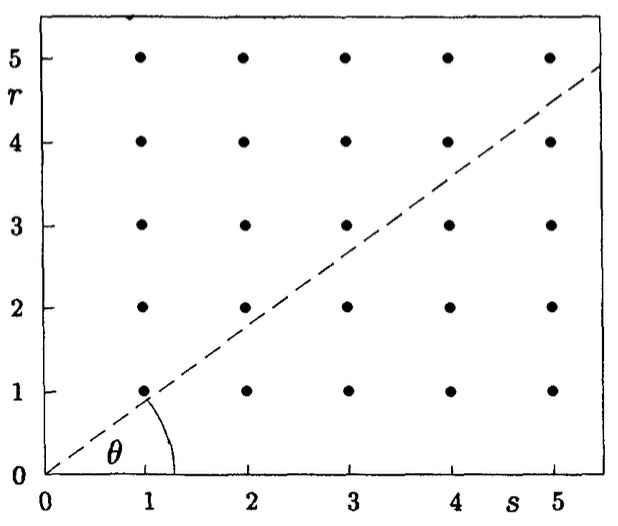
\includegraphics[width=0.25\linewidth]{pics/rs-diagram.jpg}
\end{equation*}
The dotted line has a slope $\tan \theta=-\alpha_{+} / \alpha_{-}$, fixed by the central charge $c$. 
Let $h$ be the Cartesian distance between a point $(r, s)$ and the dotted line, it can be shown that $\alpha_{r, s}= h\sqrt{\alpha_{+}^2+\alpha_{-}^2}$.
If the slope $\tan \theta$ is rational, that is, if there exist two coprime integers $p$ and $p^{\prime}$ such that $p \alpha_{-}+p^{\prime} \alpha_{+}=0$, the dotted line goes through the point $(p^{\prime}, p)$ and the conformal weights $h_{r, s}$ do not form a dense set. 
Indeed, we then have the periodicity property: $h_{r, s}=h_{r+p^{\prime}, s+p}$.
In terms of these two integers,
\begin{equation}
	c  =1-6 \frac{\left(p-p^{\prime}\right)^2}{p p^{\prime}}, \quad
	h_{r, s}  =\frac{\left(p r-p^{\prime} s\right)^2-\left(p-p^{\prime}\right)^2}{4 p p^{\prime}}.
\end{equation}
Here we assume $c\le 1$, in which case $p$ and $p'$ are positive.
One may also assume $p>p'$ without loss of generality.
It follows that
\begin{equation}
	1 \le r \le p', \quad 1\le s \le p.
\end{equation}
The symmetry $h_{r,s} = h_{p'-r,p-s}$ makes half of the rectangle redundant: $\phi_{(r,s)} = \phi_{(p'-r,p-s)}$.
Therefore, there are $(p-1)(p'-1)/2$ distict primary fields in the theory.
These finite theories are called \textit{minimal models}.
The truncated fusion rules between the fields are
\begin{equation}
	\phi_{(r, s)} \times \phi_{(m, n)}=\sum_{\substack{k=1+|r-m| \\ k+r+m=k \bmod 2}}^{k_{\max }} \quad \sum_{\substack{l=1+|s-n| \\ k+s+n=1 \bmod 2}}^{l_{\max }} \phi_{(k, l)},\quad 
	\begin{cases}
		k_{\max } =\min \left(r+m-1,2 p^{\prime}-1-r-m\right) \\
		l_{\max } =\min (s+n-1,2 p-1-s-n)
	\end{cases}
\end{equation}
If we require the representation to be unitary, all primary fields should have nonnegative conformal dimensions.
Since $p$ and $p'$ are coprime, there exist a couple of $(r_0,r_0)$ such that $p r_0-p' s_0=1$.
Accordingly, the corresponding dimension is 
\begin{equation}
	h_{r_0,s_0} = \frac{1-(p-p')^2}{4pp'} \le 0,\quad
	h_{r_0,s_0} = 0 \quad\text{when}\quad p-p'=1.
\end{equation}
Thus we can label the unitary minimal model by a single integer $m\ge 2$ ($p=m+1$, $p'=m$).


\subsection{Conformal Families}

We are now going to show that correlations of the CFT can be obtained by the operator algebra.
First consider
\begin{equation}
	\left\langle\phi_{\beta}(z,\bar z)\phi_{\alpha}(y,\bar y)\right\rangle=\frac{C_{\alpha \beta}}{(z-y)^{2 h}(\bar{z}-\bar{y})^{2 \bar h}}.
\end{equation}
Since the coefficients $C_{\alpha \beta}$ are symmetric, we are free to choose a basis of primary fields such that $C_{\alpha \beta}=\delta_{\alpha \beta}$. 
By a suitable global conformal transformation, we can always bring the points $z$ and $y$ of a correlator to $z=\infty$ and $y=0$ respectively. 
The fields are then asymptotic and the two-point function becomes a bilinear product on the Hilbert space:
\begin{equation}
	\lim_{z,\bar z \rightarrow \infty} z^{2 h} \bar z^{2\bar h}\left\langle\phi_\alpha(z,\bar z) \phi_\beta(0,0)\right\rangle 
	= \left\langle h_\alpha,\bar{h}_\alpha|h_\beta,\bar{h}_\beta \right\rangle, 
	\quad\text{where}\quad
	\left\langle h,\bar{h}\right| = \lim_{z,\bar z\rightarrow \infty} z^{2h} \bar{z}^{2\bar{h}}\langle 0|\phi_{h,\bar h}(z).
\end{equation}
The orthogonality of the highest-weight states implies the orthogonality of all the descendants of the two fields.
Invariance under scaling transformations clearly requires the operator algebra to have the following form:
\begin{equation}
	\phi_{\alpha}(z, \bar{z}) \phi_{\beta}(0,0) = \sum_{p} \sum_{\{k, \bar{k}\}} C_{\alpha\beta}^{p\{k, \bar{k}\}} z^{h_{p}-h_{\alpha}-h_{\beta}+K} \bar{z}^{\bar{h}_{p}-\bar{h}_{\alpha}-\bar{h}_{\beta}+\bar{K}} 
	\phi^{\{k, \bar{k}\}}_p(0,0),
\end{equation}
where $K=\sum_{i} k_{i}$, $\bar{K}=\sum_{i} \bar{k}_{i}$, and $\{k\}$ is a collection of indices $k_{i}$.
We take the correlator of the right-hand side with a third primary field $\phi_{\gamma}(w, \bar{w})$ of dimensions $(h_{\gamma}, \bar{h}_{\gamma})$, and send $w,\bar w$ to infinity:
\begin{equation}
	\left\langle\phi_{\gamma}\left|\phi_{\alpha}(z, \bar{z})\right| \phi_{\beta}\right\rangle =\lim _{w, \bar{w} \rightarrow \infty} w^{2 h_{\gamma}} w^{2 \bar{h}_{\gamma}}\left\langle\phi_{\gamma}(w, \bar{w}) \phi_{\alpha}(z, \bar{z}) \phi_{\beta}(0,0)\right\rangle 
	=\frac{C_{\gamma\alpha\beta}}{z^{h_{\alpha}+h_{\beta}-h_{\gamma}} \bar{z}^{\bar{h}_{\alpha}+\bar{h}_{\beta}-\bar{h}_{\gamma}}}.
\end{equation}
On the OPE side, the only contributing term is $p\{k, \bar{k}\}=\gamma\{0,0\}$, because of the orthogonality of the Verma modules. 
We conclude that $C_{\alpha\beta}^{p\{0,0\}} \equiv C_{\alpha\beta}^{p}=C_{p\alpha\beta}$.
Since the correlations of descendants are built on the correlation of primaries, we expect the coefficients $C_{\alpha\beta}^{p\{k, \bar{k}\}}$ to have the following form:
\begin{equation}
	C_{\alpha\beta}^{p \{ k, \bar{k}\}}=C_{\alpha\beta}^{p} \beta_{\alpha\beta}^{p\{k\}} \bar{\beta}_{\alpha\beta}^{p(\bar{k}\}}.
\end{equation}






\section{Canonical Quantization}










\subsection{Free Scalar Field}
The simplest example of CFT is the free scalar field $\varphi$, with the action $S = \frac{g}{2}\int d^2x\ \partial_\mu\varphi \partial^\mu \varphi$.
The propagator for 2D free boson, denoted by $K(x,y) = K(x-y)$, satisfies the differential equation: $-g \partial_r^2 K(r)  = \delta(r)$.
The propagator is then solved by $K(x,y) = -\frac{1}{4\pi g} \ln(x-y)^2 + \text{const}$.
In complex coordinates,
\begin{equation}
	\langle\varphi(z,\bar z)\varphi(w,\bar w)\rangle = -\frac{1}{4\pi g}\left[\ln(z-w) + \ln(\bar z- \bar w)\right] + \text{const}. 
\end{equation}
Concentrating on the holomorphic part, we have
\begin{equation}
	\langle\partial\varphi(z)\partial\varphi(w)\rangle = -\frac{1}{4\pi g}\frac{1}{(z-w)^2}.
\end{equation}
The stress tensor for free boson is\footnote{Note that there is a minus sign compared to the ordinary definition of Noether current. It is a commonly used convention for the stress tensor.}
\begin{equation}
\begin{aligned}
	T_{\mu\nu} = -\left(\eta_{\mu\nu} \mathcal L - \frac{\partial\mathcal L}{\partial(\partial^\mu\phi)}\partial_\nu \phi \right)
	= g\left(\partial_\mu\varphi\partial_\nu\varphi - \frac{1}{2} \eta_{\mu\nu}\partial_\rho\varphi\partial^\rho\varphi \right).
\end{aligned}
\end{equation}
The holomorphic part of it is
\begin{equation}
	T(z) = \frac{1}{4}(T_{00} - 2iT_{01} - T_{11}) = -2\pi g \partial_z\varphi \partial_z\varphi.
\end{equation}
Now we are considering the quantum version of the stress tensor.
We shall use the normal-ordered form
\begin{equation}
	T(z) = -2\pi g \normord{\partial_z\varphi(z) \partial_z\varphi(z)}.
\end{equation}
For free field, it is just
\begin{equation}
	T(z) = -2\pi g \lim_{w\rightarrow z}\left[\partial\varphi(z)\partial\varphi(w)-\langle\partial\varphi(z)\partial\varphi(w)\rangle\right].
\end{equation}
To compute the OPE for stress tensors, consider
\begin{equation}
\begin{aligned}
	T(z)T(w) 
	&= (2\pi g)^2 \normord{\partial_z\varphi(z) \partial_z\varphi(z)} \normord{\partial_z\varphi(w) \partial_z\varphi(w)} \\
	&\sim (2\pi g)^2 \left[\frac{2}{(4\pi g)^2}\frac{1}{(z-w)^4} - \frac{4}{4\pi g}\frac{\normord{\partial_z\varphi(z)\partial_z\varphi(w)}}{(z-w)^2}\right] \\
	&= \frac{1/2}{(z-w)^4} + \frac{4\pi g}{(z-w)^2}\normord{\partial_z\varphi(z)\partial_z\varphi(w)}.
\end{aligned}
\end{equation}
In the second equation, the first term is the result of two contractions, and the second the result of single contraction.

\paragraph*{Normal Ordering}
We digress a little bit to discuss the normal ordering.
The normal ordering handles the divergent comes from the contact of two field.
In general, the OPE for $A(z)$ and $B(w)$ has the form
\begin{equation}
	A(z) B(w) = \sum_{n=-\infty}^N \frac{\{AB\}_n(w)}{(z-w)^n}
\end{equation}
The order ordering result is $\normord{AB}=\{AB\}_0$.
Our definition of the contraction is generalized to include all the singular terms of the OPE:
\begin{equation}
	\wick{\c1{A}(z) \c1{B} (w)} \equiv \sum_{n=1}^{N} \frac{\{A B\}_{n}(w)}{(z-w)^{n}}.
\end{equation}
Hence the above expression for $\normord{A B}(w)$ may be rewritten as
\begin{equation}
	\normord{A B}(w) = \lim _{z \rightarrow w}[A(z) B(w)- \wick{\c1 A(z) \c1 B}(w)],
\end{equation}
and the OPE of $A(z)$ with $B(w)$ is expressed as
\begin{equation}
	A(z) B(w) = \wick{\c1 A(z) \c1 B}(w)+ \normord{A(z) B(w)},
\end{equation}
where $\normord{A(z) B(w)}$ stands for the complete sequence of regular terms whose explicit forms can be extracted from the Taylor expansion of $A(z)$ around $w$ :
\begin{equation}
	\normord{A(z) B(w)} = \sum_{k \geq 0} \frac{(z-w)^{k}}{k !}\normord{\partial^{k} A B}(w).
\end{equation}
Now if we take $A=B=\partial\varphi$, we have
\begin{equation}
\begin{aligned}
	 \frac{4\pi g}{(z-w)^2} \normord{\partial\varphi(z) \partial\phi(w)} 
	 &= 4\pi g \sum_{k \geq 0} \frac{(z-w)^{k-2}}{k !}\normord{\partial^{k} \partial\varphi \partial\varphi}(w) \\
	 &\sim - \frac{2T(w)}{(z-w)^2} + \frac{4\pi g \normord{\partial^2\varphi \partial\varphi}(w)}{z-w} 
	 = - \frac{2T(w)}{(z-w)^2} - \frac{\partial T(w)}{z-w}.
\end{aligned}
\end{equation}
We thus know the OPE for free boson:
\begin{equation}
	T(z) T(w) = \frac{1/2}{(z-w)^4} - \frac{2T(w)}{(z-w)^2} - \frac{\partial T(w)}{z-w}.
\end{equation}
The central charge for free boson is $1$.


\paragraph*{Quantization on the Cylinder}
Now we adopt the normalization $g = 1/4\pi$, the Fourier expansion of the field is
\begin{equation}
	\varphi(x, t) =\sum_{n} e^{2 \pi i n x / L} \varphi_{n}(t), \quad
	\varphi_{n}(t) =\frac{1}{L} \int d x e^{-2 \pi i n x / L} \varphi(x, t).
\end{equation}
The Lagrangian becomes
\begin{equation}
	\frac{L}{8\pi} \sum_{n}\left[\dot{\varphi}_{n} \dot{\varphi}_{-n}-\left(\frac{2 \pi n}{L}\right)^{2} \varphi_{n} \varphi_{-n}\right],
\end{equation}
Introducing the momentum $\pi_n=\frac{1}{4\pi} L \dot{\varphi}_{-n}$, $\left[\varphi_{n}, \pi_{m}\right]=i \delta_{n m}$, the Hamiltonian is
\begin{equation}
	H=\frac{2\pi}{L} \sum_{n}\left[\pi_{n} \pi_{-n}+ \left(\frac{n}{2}\right)^2 \varphi_{n} \varphi_{-n}\right].
\end{equation}
The canonical ladder operators are
\begin{equation}
	\tilde a_n = \frac{1}{\sqrt{|n|}}\left(\frac{|n|}{2}\varphi_n + i\pi_{-n}\right), \quad
	\tilde a_n^\dagger = \frac{1}{\sqrt{|n|}}\left(\frac{|n|}{2}\varphi_{-n} - i\pi_{n}\right),
\end{equation}
which satisfies the canonical commutation relation $[\tilde a_n, \tilde a_m^\dagger] = \delta_{mn}$, and the Hamiltonian becomes the diagonal form
\begin{equation}
	H = \frac{2\pi}{L} \sum_n |n| \left(\tilde a_n^\dagger \tilde a_n + \frac{1}{2} \right).
\end{equation}
However, ladder operator does not work for the zero modes.
We can instead define the operator
\begin{equation}
	a_{n} = \begin{cases}
		-i \sqrt{n} \tilde{a}_{n} & (n>0) \\
		i \sqrt{-n} \tilde{a}_{-n}^{\dagger} & (n<0)
	\end{cases}
	= -i\frac{n}{2} \varphi_n + \pi_{-n}, \quad
	\bar a_{n} = \begin{cases}
		-i \sqrt{n} \tilde{a}_{-n} & (n>0) \\
		i \sqrt{-n} \tilde{a}_{n}^{\dagger} & (n<0)
	\end{cases}
	= -i\frac{n}{2} \varphi_{-n} + \pi_{n}.
\end{equation}
The commutation relations are $\left[a_{n}, a_{m}\right]=n \delta_{n+m}$, $\left[a_{n}, \bar{a}_{m}\right]=0$, and $\left[\bar{a}_{n}, \bar{a}_{m}\right]=n \delta_{n+m}$.
The Hamiltonian is then expressible as
\begin{equation}
	H=\frac{2\pi}{L} \pi_{0}^{2}+\frac{2 \pi}{L} \sum_{n > 0}\left(a_{-n} a_{n}+\bar{a}_{-n} \bar{a}_{n}\right).
\end{equation}
The field mode $\varphi_n$ for $n\ne 0$ is $\varphi_n = \frac{i}{n} (a_n-\bar a_{-n})$.
The field $\varphi(x,t)$ is
\begin{equation}
	\varphi(x,t) = \varphi_0(t) + \sum_{n\ne 0} \frac{i}{n} \left[a_n(t)-\bar a_{-n}(t)\right] e^{-2\pi i n x/L}.
\end{equation}
Note that
\begin{equation}
\begin{aligned}
	\partial_t \phi_0 &= i [H,\varphi_0] = -i\frac{4\pi}{L} \pi_0 [\phi_0, \pi_0] = \frac{4\pi}{L}\pi_0, \\
	\partial_t a_n &= i[H, a_n] = -i \frac{2\pi}{L} n a_n, \\
	\partial_t \bar a_n &= i[H, \bar a_n] = -i \frac{2\pi}{L} n \bar a_n.
\end{aligned}
\end{equation}
We thus have
\begin{equation}
	\varphi(x, t)=\varphi_{0}+\frac{4\pi}{L} \pi_{0} t + \sum_{n \neq 0} \frac{i}{n}\left[a_{n} e^{2 \pi i n(x-t) / L}-\bar{a}_{-n} e^{2 \pi i n(x+t) / L}\right].
\end{equation}
We can now first go to Euclidean space ($it \rightarrow \tau$), and then change to the complex variables $z = e^{2\pi(\tau-ix)/L}$, $\bar z = e^{2\pi(\tau+ix)/L}$.
We then obtain the expression
\begin{equation}
	\varphi(z, \bar{z})=\varphi_{0}-\frac{i}{4 \pi g} \pi_{0} \ln (z \bar{z})+\frac{i}{\sqrt{4 \pi g}} \sum_{n \neq 0} \frac{1}{n}\left(a_{n} z^{-n}+\bar{a}_{n} \bar{z}^{-n}\right),
\end{equation}
where the holomorphic part and antiholomorphic part decouples.
We know $\varphi$ itself is not a primary field, but the $i\partial\varphi$ is:
\begin{equation}
	i\partial\varphi(z) = \frac{\pi_0}{z} + \sum_{n\ne 0} a_n z^{-n-1}.
\end{equation}
If we define $a_0 \equiv \bar a_0 \equiv \pi_0$,
\begin{equation}
	i\partial\varphi(z) = \sum_n a_n z^{-n-1}.
\end{equation}





\section{Entaglement Entropy}

This section focus on the entanglement entropy $S\equiv \tr \rho \ln \rho$.
We denote the complete set of local field operators as $\{\phi_x\}$, the density operator can be written as
\begin{equation}
	\rho\left(\{\phi_x\}|\{\phi'_{x'}\}\right)
	= \frac{1}{Z(\beta)}\left\langle\{\phi_x\}\right| e^{-\beta H}\left|\{\phi'_{x'}\}\right\rangle, \quad 
	Z(\beta) = \Tr e^{-\beta H}.
\end{equation}
This can be expressed as the path integral
\begin{equation}
	\rho(\{\phi_{x}\}|\{\phi_{x^{\prime}}^{\prime}\}) = \frac{1}{Z} \int D \phi_{y, \tau} \prod_{x^{\prime}} \delta\left(\phi_{y, 0}-\phi_{x^{\prime}}^{\prime}\right) \prod_{x} \delta\left(\phi_{y, \beta}-\phi_{x}\right) \mathrm{e}^{-S_{E}}
\end{equation}
defined on the manifold with imaginary time interval $(0,\beta)$.
We assume the system is in a pure state, the reduced density matrix for the subsystem is obtained by taking the partial trace.
In the path-integral formalism, the density matrix can be represented by a cylinder with boundaries:
\begin{equation*}
	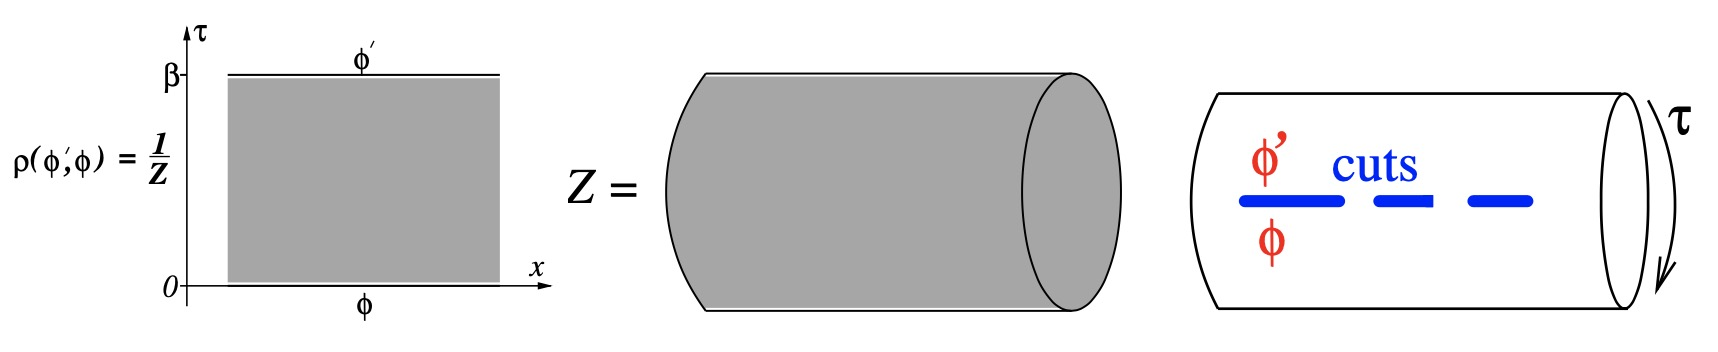
\includegraphics[width=0.7\linewidth]{pics/manifold.jpg}
\end{equation*}
We see that the reduced density matrix $\rho_A$ is obtained by sewing together only those points x which are not in $A$.
If we consider the ground state, just take $\beta$ to infinity and the manifold becomes the infinite plane.



\subsection{Replica method and twisted fields}
A closely related quantity for entanglement entropy is the Renyi entropy $S_A^{(n)} = \frac{1}{1-n} \ln \tr \rho_A^n$.
If the Renyi entropy is an analytic function of $n$, then the (von Neumann) entropy can be obtained by first considering the integer $n$ case and then taking the analytic continuation $n\rightarrow 1$:
\begin{equation}
	S_A = \lim_{n\rightarrow 1}S_A^{(n)} = \lim_{n\rightarrow1} Z\left[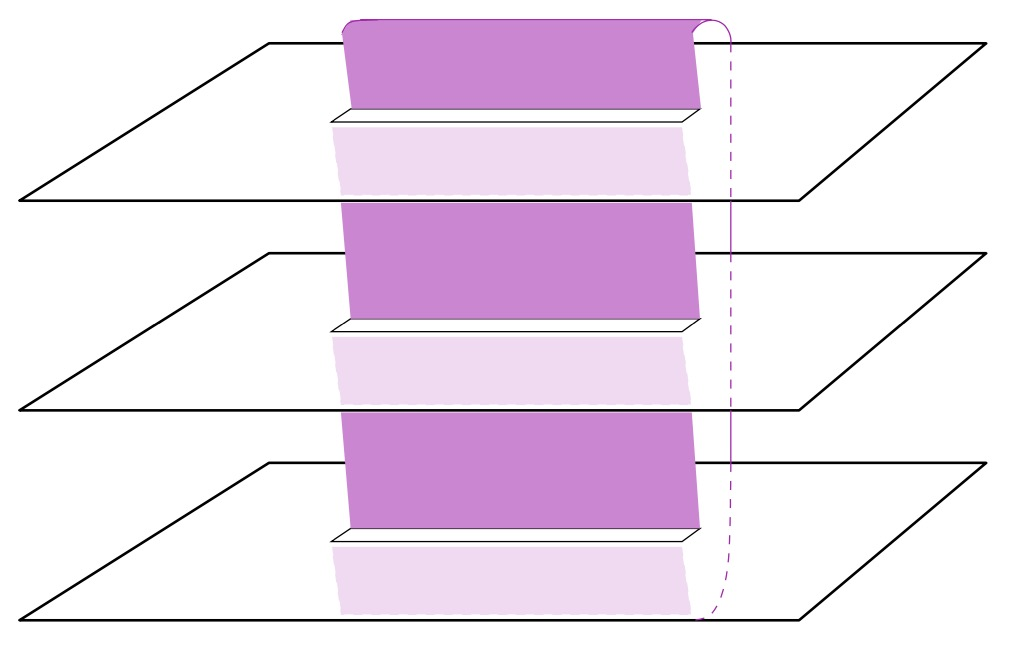
\includegraphics[align=c,width=0.18\linewidth]{pics/Riemannsurf.jpg}\right],
\end{equation}
where we have mapped the problem to the partition function of a ``replica" system located on an $n$-sheeted Riemann surface.
Each layer corresponds to a different copy of the field.
The bulk theory of the system is just $n$ copies of the original Lagrangian, while the boundary condition introduced a branch cut to the theory.

Cardy et al. proposed that the field theory can be well described by inserting the \textit{twist fields} $\mathcal T_n$, $\tilde{\mathcal T}_n$ to each of the n disconnected sheets.
The partition function and other expectation values (on a single sheet) can be expressed as:
\begin{equation}
	Z_n = \langle \mathcal{T}_n(u) \tilde{\mathcal{T}}_n(v)\rangle, \quad
	\langle O(x,\tau)\rangle = \frac{1}{Z_n}\langle\mathcal{T}_n(u) \tilde{\mathcal{T}}_n(v) O(x,\tau) \rangle.
\end{equation}
One of the most important operators in the conformal field theory is the stress tensor $T(z)$.
The expectation value for stress tensor can be obtained by considering the conformal mapping
\begin{equation}
	z \rightarrow w(z) = \left(\frac{z-u}{z-v}\right)^{\frac{1}{n}}.
\end{equation} 
One can check that $w$ maps the Riemann surface to a single complex plane.
The stress tensors on different manifolds are related by
\begin{equation}
	\langle T(z) \rangle = \left(\frac{d w}{d z}\right)^{2} \langle T(w)\rangle + \frac{c}{12}\{w, z\},
\end{equation}
where the Schwarzian derivative $\{z, w\}$ is
\begin{equation}
	\{w,z\} = \left(\frac{dw}{dz}\right)^{-2} \left[\frac{d^3 w}{dz^3}\frac{dw}{dz} - \frac{3}{2}\left(\frac{d^2 w}{dz^2}\right)^2\right] 
	= \frac{1}{2}\left(1-\frac{1}{n^2}\right)\frac{(u-v)^2}{(z-u)^2(z-v)^2}.
\end{equation}
The stress tensor on the complex plane is zero: $\langle T(w)\rangle=0$, so that on the Riemann surface is
\begin{equation}
	\frac{\langle\mathcal{T}_n(u) \tilde{\mathcal{T}}_n(v) T(z) \rangle}{\langle\mathcal{T}_n(u) \tilde{\mathcal{T}}_n(v) \rangle} 
	= \frac{c}{24}\left(1-\frac{1}{n^2}\right)\frac{(u-v)^2}{(z-u)^2(z-v)^2}.
\end{equation}
If we assume the twist field is primary, with dimension $d_n$, the two-point function is\footnote{We focus on the holomorphic part and assume the anti-holomorphic part has the same dimensionality. Also, note that we have chosen a proper normalization for the twist fields.}
\begin{equation}
	\langle\mathcal{T}_n(u) \tilde{\mathcal{T}}_n(v) \rangle
	= (u-v)^{-2d_n}.
\end{equation}
And we also have the conformal Ward identity
\begin{equation}
	\langle\mathcal{T}_n(u) \tilde{\mathcal{T}}_n(v) T(z) \rangle
	= \left[\frac{\partial_u}{z-u} +\frac{d_n}{(z-u)^{2}}+\frac{\partial_v}{z-v} + \frac{d_n}{(z-v)^{2}}\right] \left\langle\mathcal{T}_{n}(u) \tilde{\mathcal{T}}_{n}(v)\right\rangle 
	= d|u-v|^{2-2d}.
\end{equation}
Together we know $d_n = \frac{c}{24}\left(1-n^{-2}\right)$.


\subsection{Equilibrium entaglement entropy}
We first consider the zero-temperature, ground-state entanglement entropy.
Note that the partition function for the replica system is related to the Renyi entropy by:
\begin{equation}
	\frac{Z_n}{Z^n} \propto \Tr \rho_A^n = c_n \left|\frac{u-v}{a}\right|^{-4n d_n},
\end{equation}
where $a$ is the UV cutoff introduced by $Z^n$.
The $n$-th order Renyi entropy is then
\begin{equation}
	S^{(n)}_A = \frac{c}{6}\left(1+\frac{1}{n}\right) \ln \left|\frac{u-v}{a}\right| + \frac{\ln c_n}{1-n}.
\end{equation}
As discussed, the entanglement entropy is obtained by taking the limit
\begin{equation}
	\lim_{n\rightarrow 1} S^{(n)}_A = \frac{c}{3}\ln\left|\frac{u-v}{a}\right| - c'_1.
\end{equation}
We thus obtained the entanglement entropy behavior of the single interval with length $l$:
\begin{equation}
	S_A = \frac{c}{3}\ln\frac{l}{a} + O(1).
\end{equation}

We can also obtain the exact form of entanglement entropies for finite size or finite temperature, using a special conformal mapping that map the complex plane to an infinite cylinder with circumference $\beta$:
\begin{equation*}
	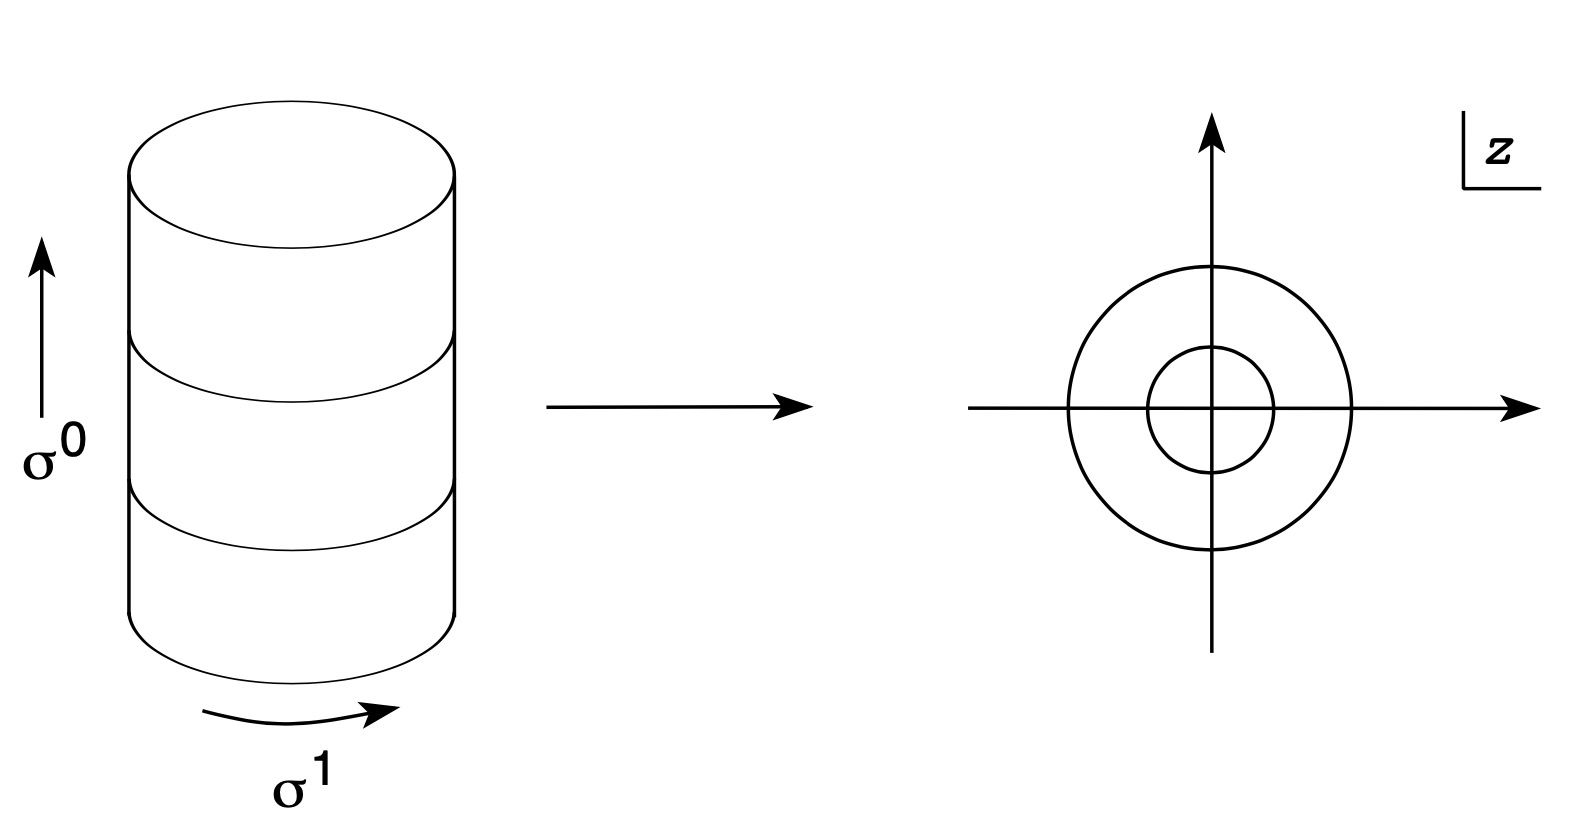
\includegraphics[width=0.45\linewidth]{pics/cyldrmap.jpg}
\end{equation*}
Specifically, $w$ and $z$ are related by:
\begin{equation}
	w = \frac{\beta}{2\pi} \ln z, \quad
	z = \exp\left(\frac{2\pi w}{\beta}\right).
\end{equation}
There are different ways to place $u$ and $v$.
If we place them along the radius, their image lies parallel to the cylinder's axis (the images are denoted as $w_1$ and $w_2$ respectively).
This corresponds to the infinite chain with a finite temperature.
The two-point function is
\begin{equation}
\begin{aligned}
	\langle \mathcal{T}_n(w_1) \tilde{\mathcal T_n}(w_2)\rangle
	&= \left[w'(z_1)w'(z_2)\right]^{-d_n} \langle \mathcal{T}_n(z_1) \tilde{\mathcal T_n}(z_2)\rangle \\
	&= \exp \left[\frac{2\pi}{\beta} d_n(w_1+w_2)\right] \left[\exp\left(\frac{2\pi}{\beta} w_1\right)-\exp\left(\frac{2\pi}{\beta} w_2\right)\right]^{-2d_n} \\
	&= \left\{2\sinh\left[\frac{\pi(w_1-w_2)}{\beta}\right]\right\}^{-2d_n}.
\end{aligned}
\end{equation}
Similarly, we have
\begin{equation}
	\Tr \rho_A^n = c_n \left[\frac{2}{b(\beta)}\sinh\left(\frac{\pi l}{\beta}\right)\right]^{-4nd_n}.
\end{equation}
The $b(\beta)$ is a $\beta$-dependent cutoff that should have the asymptotic behavior
\begin{equation}
	\lim_{\beta \rightarrow \infty} \frac{2}{b(\beta)}\sinh\left(\frac{\pi l}{\beta}\right) = \frac{l}{a} 
	\quad \Longrightarrow \quad
	b(\beta) = \frac{2\pi a}{\beta}.
\end{equation}
Thus the Renyi entropy for the replica system is
\begin{equation}
	S_A^{(n)} = \frac{c}{6}\left(1+\frac{1}{n}\right) \ln \left[\frac{\beta}{\pi a}\sinh\left(\frac{\pi l}{\beta}\right)\right] + \frac{\ln c_n}{1-n}.
\end{equation}
The entanglement entropy from the replica limit is
\begin{equation}
	S_A = \frac{c}{3} \ln \left[\frac{\beta}{\pi a}\sinh\left(\frac{\pi l}{\beta}\right)\right] + O(1).
\end{equation}

Apart from this, we can also place $u$ and $v$ on the same circle so that their image is perpendicular to the axis of the cylinder.
The calculation carries out without a change, but now $\beta$ is regarded as the system size (periodic boundary condition) while the temperature is zero.
We usually denote the size of the finite chain as $L$, so the finite-size result is:
\begin{equation}
	S_A = \frac{c}{3} \ln \left[\frac{L}{\pi a}\sinh\left(\frac{\pi l}{L}\right)\right] + O(1).
\end{equation}




\section{Conformal Bootstrap}

For four-point functions, the general solution is
\begin{equation}
	Z = \left(\prod_{i<j} z_{ij}^{-h_{i j}}\right) G\left(\frac{z_{12}z_{34}}{z_{13}z_{24}}\right),\quad
	\text{where } h_{ij} = h_{ji},\ \sum_{i\ne j} h_{ij} = 2\Delta_i. 
\end{equation}
Here $G$ is an arbitrary function. 
The six numbers $h_{ij}$ ($i<j$) are subject to only four equations, leaving two undetermined combinations. 
Changing these combinations amounts to a redefinition $G(z) \rightarrow z^\lambda(1-z)^\mu G(z)$.
So the three global Ward identities effectively reduce the four-point function to a function of one variable $G$-equivalently, we can set $z_2=0, z_3=\infty, z_4=1$, and recover the four-point function from its dependence on $z_1$ alone:
\begin{equation}
	G(z)=\left\langle \phi_{\Delta_1}(z) \phi_{\Delta_2}(0) \phi_{\Delta_3}(\infty) \phi_{\Delta_4}(1)\right\rangle,\quad\text{where}\ \ 
	\phi_{\Delta}(\infty)=\lim _{z \rightarrow \infty} z^{2 \Delta} \phi_{\Delta}(z).
\end{equation}

\end{document}


